\documentclass[aps,twocolumn,secnumarabic,balancelastpage,amsmath,amssymb,nofootinbib]{revtex4}

% Documentclass Options
    % aps, prl stand for American Physical Society and Physical Review Letters respectively
    % twocolumn permits two columns, of course
    % nobalancelastpage doesn't attempt to equalize the lengths of the two columns on the last page
        % as might be desired in a journal where articles follow one another closely
    % amsmath and amssymb are necessary for the subequations environment among others
    % secnumarabic identifies sections by number to aid electronic review and commentary.
    % nofootinbib forces footnotes to occur on the page where they are first referenced
        % and not in the bibliography
    % REVTeX 4 is a set of macro packages designed to be used with LaTeX 2e.
        % REVTeX is well-suited for preparing manuscripts for submission to APS journals.


\usepackage{lgrind}        % convert program listings to a form includable in a LaTeX document
\usepackage{chapterbib}    % allows a bibliography for each chapter (each labguide has it's own)
\usepackage{color}         % produces boxes or entire pages with colored backgrounds
\usepackage{graphics}      % standard graphics specifications
\usepackage[pdftex]{graphicx}      % alternative graphics specifications
\usepackage{longtable}     % helps with long table options
\usepackage{epsf}          % old package handles encapsulated post script issues
\usepackage{bm}            % special 'bold-math' package
%\usepackage{asymptote}     % For typesetting of mathematical illustrations
\usepackage{thumbpdf}
\usepackage[colorlinks=true]{hyperref}  % this package should be added after all others
                                        % use as follows: \url{http://www.usm.maine.edu/~pauln/MainSite/PHY240.html}
%
% And now, begin the document...
% Students should not have to alter anything above this line
%
\begin{document}
\title{Undergraduate Radiation Experiments: \\ Optimizing a Geiger-Muller Tube \& Measuring Absorption}
\author         {A. Knight \& N. Anna}
\email          {alexander.knighr@maine.edu \& nicholas.anna@maine.edu}
\date{\today}
\affiliation{USM Department of Physics}


\begin{abstract}
The following contains a summary of two experiments involving radiation at the undergraduate physics level. It aims to provide enough of a summary to allow students at such a level to confirm experimental results and improve upon experiment design. Upon receipt of a digital Geiger meter, the need arose to design two introductory experiments involving the equipment. The tasks that were chosen were finding the optimum voltage for the Geiger-Muller tube and testing the absorptivity of differing materials with varying sources.
\end{abstract}

\maketitle

\section{Problem and Relevant Theory}
\subsection{Detecting Radiation}
To conduct any sort of investigation of radiation,  a reliable method to determine quantities of radiation present is needed. Exploiting the fact that radiation incident on a gas atom can knock an electron loose, Walther Muller developed a method to count these electrons \cite{introGeiger}. It involves a sealed metal tube filled with an inert gas that is easy to ionize. A wire, which is insulated from the exterior of the cylinder, is passed through the center of the tube, and a voltage is applied to the two components of the tube. This voltage pulls the electrons towards the center wire, and if strong enough it will give the electrons enough energy to knock off an electron from the next gas particle it collides with\cite{townsend}. This cascade of electrons will produce a detectable current when it reaches the center wire.

The sensitivity of the tube is determined by the voltage applied to it. However, there are some voltage regions which have a flat response and give consistent readings as shown in Fig \ref{fig:countRegion}.

\begin{figure}[b]
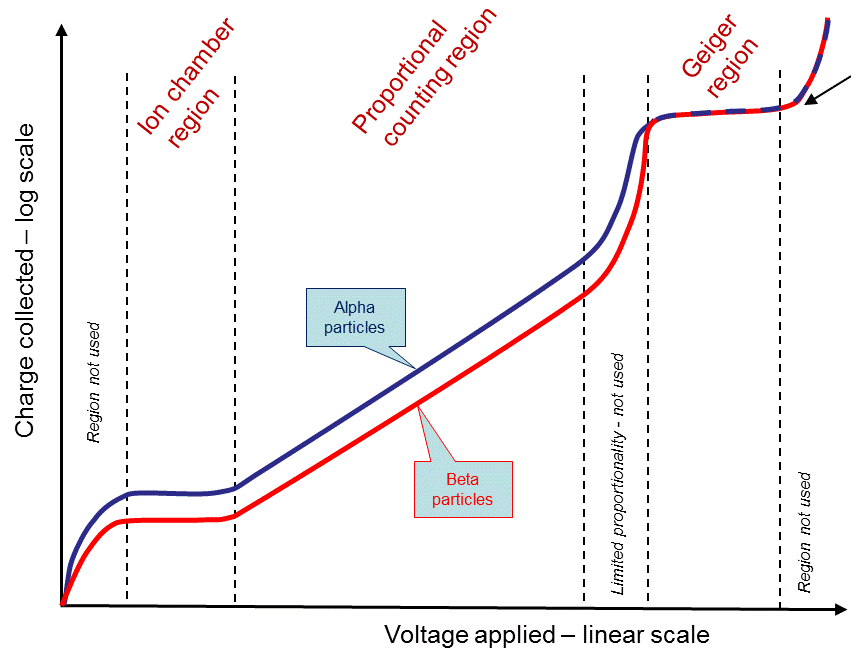
\includegraphics[width=9cm]{countRegion}
\caption{The expected sensitivity of the detector to differing particle types at varying voltages. \textit{source: wikimedia commons}}
\label{fig:countRegion}
\end{figure}

There are several short comings to this method. The Geiger-Muller tube cannot discern what type of radiation (alpha, beta, or gamma) is incident on the tube. The method also fails to give any information about the energy level of the incident radiation.

\subsection{Absorbing Radiation}
Another immediate concern while working with radiation is to protect lab personell. To this end, we will test how well materials of varying densities absorb it.  While this lab deals with small sources in sealed containers, knowing the absorptivity of materials for various sources is instrumental in safety planning. This paper will seek to find a model for this behaviour.

%%%%%%%%%%%%%%%%%%%%%%%%%%%%%%%%%%%%%%%%%%%%%%%%%%%%%%%%%%%%%%%%%%%%%%%%%%%%%
\section{Experimental Setup}
\subsection{G-M Tube}
The method used to determine the best voltage to take readings was to measure the background radiation and the radiation from several different sources at a range of voltages allowed by our device. The distance from the source to the detector is trivial, so long as it stays fixed throughout the experiment. Using Co-60, Cs- 137 and Sr- 90 as sources, the radiation count from a fixed time period was recorded 5 times at each voltage. This was used to compute the average rate of detected radiation as well as the standard deviation of this average.

\subsection{Absorption Setup}
For this portion of the experiment Co-60 was chosen as the source and aluminum and lead, the shielding materials. Again placing the source at a fixed distance from the detector, a series of raw count rate readings are taken from the source. Then, for each varying thicknesses of shielding material, a subsequent series of count rate readings are taken.

%%%%%%%%%%%%%%%%%%%%%%%%%%%%%%%%%%%%%%%%%%%%%%%%%%%%%%%%%%%%%%%%%%%%%%%%%%%%%
\section{Data Presentation \& Analysis}
\subsection{Count Rate vs. Voltage}
The rates of detection were recorded over a 20 second interval, with each element. Figure \ref{fig:RateVsVolt} shows the results with the corresponding 95\% CI of the average rate. For each different type of emitter the response rate of the detector plateaus around 980v. This will be chosen for the voltage for follow on experimentation. It is interesting to note, at voltages close to lower end of the useful range, it was difficult to take a reading because the detector would work normally for several seconds, and then freeze. This is likely because the gas in the tube saturates with positive ions, as the voltage isn't strong enough to pull them to the container wall fast enough to deionize them at the same rate new incident radiation would be detected.
\begin{figure}[h]
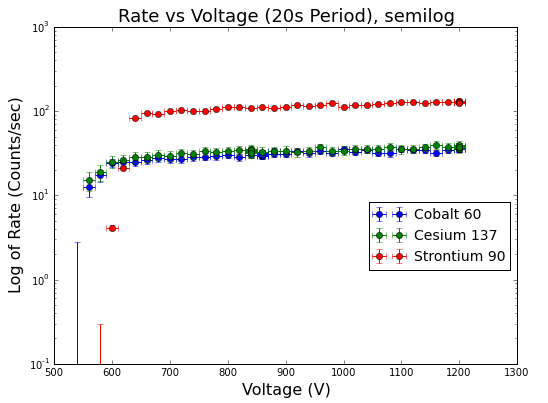
\includegraphics[width=9cm]{RateVsVolt}
\caption{The ion region zone of the Geiger-Muller tube, as demonstrated with several radioactive sources.}
\label{fig:RateVsVolt}
\end{figure}
\subsection{Absorptivity}
First we tested lead varying in thickness from 0 cm to 1.2 cm thick. The thickness of these plates was verified with a micrometer. The average rate of 5 runs of 60 seconds and the 95\% CI of this average is shown in Figure \ref{fig:leadAbsorbRaw}. Also shown is the best fit decay line. The decay pattern observed in the data appeals to intuition because it seems reasonable that the rate of incident radiation $I$ which passes through a tiny increment $dx$ of material ought to change proportionally to the thickness, rate of incident radiation, and a factor of the material we shall call $\mu$ with units $\frac{1}{cm}$. This is expressed as $$\frac{dI}{dx} = -\mu I$$
which is the familiar differential equation giving the solution
\begin{equation}
I(x) = I_oe^{-\mu x}
\label{eqn:incidentAfterX}
\end{equation}

\begin{figure}
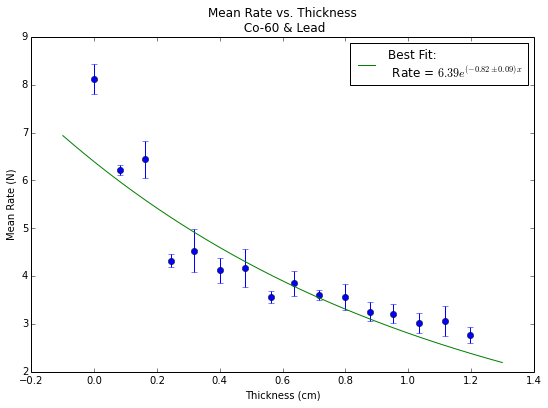
\includegraphics[width=9cm]{leadAbsorbRaw}
\caption{Rate of incident radiation from Co-60 after transmission through a thickness of lead. Shown with best fit exponential decay.}
\label{fig:leadAbsorbRaw}
\end{figure}

We found we got a much narrower uncertainty on $\mu$ when we disregarded the first three data points of our series. This can be explained by reasoning through the $\beta ^-$ decay process \cite{Co60}. The atom goes through decay and ejects an electron from the nucleus. Addtionally, the remaining valence electron of the new atom makes two subsequent downward transitions, releasing two $\gamma$ particles. The released electron is stopped after a very small qauntity of lead, leaving us with just the gamma rays from there on.









%%%%%%%%%%%%%%%%%%%%%%%%%%%%%%%%%%%%%%%%%%%%%%%%%%%%%%%%%%%%%%%%%%%%%%%%%%%%%
\section{Conclusions}
\subsection{Optimum G-M Tube Voltage}The counting equipment used for this experiment did not provide adequate voltage to reach to the Geiger region. However, it did comfortably reach the ion chamber zone, as evidenced by the flat response to the provided sources with differing voltages. We were unable to determine the upper bound of the ion chamber region, due to equipment limitations. However, we were able to determine that 980v is well within the ion chamber zone and is a good voltage to take readings at.

\subsection{Linear X-ray Attenuation}
Our model of the absorption of radiation in a solid being an exponential decay not only fits our data, but is consistent with the well known properties of radiation \cite{atten}. We observed a value of $\mu_{Pb} = 0.44 \pm 0.04 \frac{1}{cm}$. The average energy of gamma radiation emitted by Co-60 is $1.25$ MeV and lead has a well-known value of $\mu_{Pb} =  0.67 \frac{1}{cm}$ for photons of this energy.  This represents a 34\% error. Taking more data points could help resolve this error. This would be greatly eased by scripting the detector to run samples and record them in the absence of the experimenter \cite{scriptedExperiment}.

The readings collected for aluminum were inconclusive due to having too small a decrease in radiation compared with the variance of our readings. This could be remedied in future experiments by using thicker increments of aluminum shielding material. The measured attenuation coefficient and 95\% CI is $\mu_{Al} = 0.38 \pm 0.05$. This is a 157\% error from the NIST value.


\begin{figure}[h]
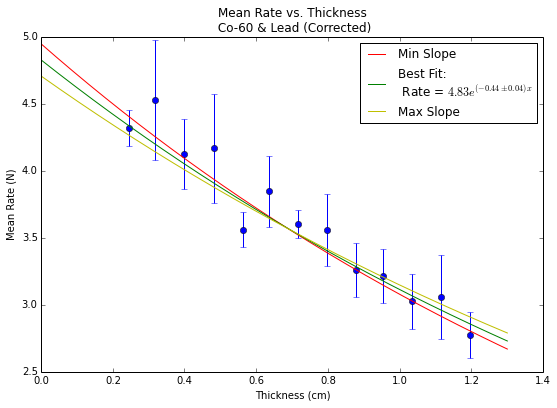
\includegraphics[width=9cm]{conclusionImage}
\label{fig:conclusionImage}
\caption{The best fit line and its 95\% CI. This data excludes the first three data points.}
\end{figure}

%%%%%%%%%%%%%%%%%%%%%%%%%%%%%%%%%%%%%%%%%%%%%%%%%%%%%%%%%%%%%%%%%%%%%%%%%%%%%
% Place all of the references you used to write this paper in a file
% with the same name as following the \bibliography command
%%%%%%%%%%%%%%%%%%%%%%%%%%%%%%%%%%%%%%%%%%%%%%%%%%%%%%%%%%%%%%%%%%%%%%%%%%%%%

\bibliographystyle{plain}
\nocite{*}
\bibliography{radiationReportBib}

\end{document}
